\documentclass[tikz,border=2pt]{standalone}
\usepackage{amsmath}
\usepackage{pgfplots}
\pgfplotsset{compat=1.18}
\usetikzlibrary{arrows.meta}
\begin{document}
% Schematic RStudio window: script editor, console, environment and help panes; Run sends a
% script line to the console, the stored object appears in the environment pane.
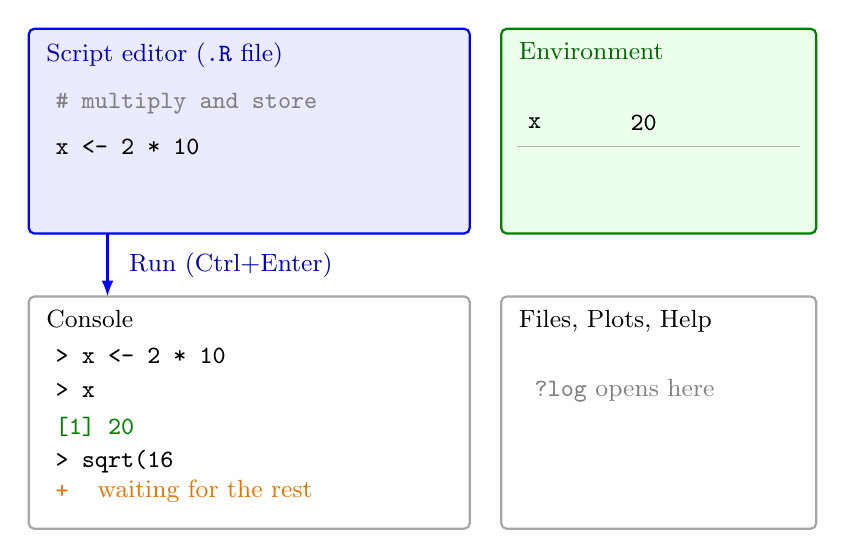
\begin{tikzpicture}[font=\small, >={Latex[length=2mm]},
  pane/.style={draw, rounded corners=2pt, thick},
  code/.style={anchor=west, font=\small\ttfamily, inner sep=1pt}]
  % script editor
  \draw[pane, blue, fill=blue!8] (0,3.4) rectangle (5.6,6);
  \node[anchor=north west, blue!70!black] at (0.1,5.95) {Script editor (\texttt{.R} file)};
  \node[code, gray] at (0.3,5.05) {\# multiply and store};
  \node[code] at (0.3,4.5) {x <- 2 * 10};
  % console
  \draw[pane, gray!70] (0,-0.35) rectangle (5.6,2.6);
  \node[anchor=north west] at (0.1,2.55) {Console};
  \node[code] at (0.3,1.85) {> x <- 2 * 10};
  \node[code] at (0.3,1.4) {> x};
  \node[code, green!50!black] at (0.3,0.95) {[1] 20};
  \node[code] at (0.3,0.5) {> sqrt(16};
  \node[code, orange!90!black] at (0.3,0.12) {+};
  \node[anchor=west, orange!90!black] at (0.75,0.12) {waiting for the rest};
  % run arrow
  \draw[->, thick, blue] (1.0,3.4) -- (1.0,2.6);
  \node[anchor=west, blue!70!black] at (1.15,3.0) {Run (Ctrl+Enter)};
  % environment
  \draw[pane, green!50!black, fill=green!8] (6,3.4) rectangle (10,6);
  \node[anchor=north west, green!40!black] at (6.1,5.95) {Environment};
  \node[code] at (6.3,4.8) {x};
  \node[code] at (7.6,4.8) {20};
  \draw[gray!60] (6.2,4.5) -- (9.8,4.5);
  % help and plots
  \draw[pane, gray!70] (6,-0.35) rectangle (10,2.6);
  \node[anchor=north west] at (6.1,2.55) {Files, Plots, Help};
  \node[anchor=west, gray] at (6.3,1.4) {\texttt{?log} opens here};
\end{tikzpicture}
\end{document}
